
% Note that the a4paper option is mainly intended so that authors in
% countries using A4 can easily print to A4 and see how their papers will
% look in print - the typesetting of the document will not typically be
% affected with changes in paper size (but the bottom and side margins will).
% Use the testflow package mentioned above to verify correct handling of
% both paper sizes by the user's LaTeX system.
%

\documentclass[12pt,journal,compsoc]{IEEEtran}

% Used to generate links, can be removed for final version
\usepackage{hyperref}
%used for \cref
\usepackage{cleveref}

\usepackage{listings}

\newcommand{\shellcmd}[1]{\\\texttt{\footnotesize\# #1}}

% *** CITATION PACKAGE ***
\usepackage{cite}
\usepackage{newclude}

% cite.sty was written by Donald Arseneau
% V1.6 and later of IEEEtran pre-defines the format of the cite.sty package
% \cite{} output to follow that of IEEE. Loading the cite package will
% result in citation numbers being automatically sorted and properly
% "compressed/ranged". e.g., [1], [9], [2], [7], [5], [6] without using
% cite.sty will become [1], [2], [5]--[7], [9] using cite.sty. cite.sty's
% \cite will automatically add leading space, if needed. Use cite.sty's
% noadjust option (cite.sty V3.8 and later) if you want to turn this off
% such as if a citation ever needs to be enclosed in parenthesis.
% cite.sty is already installed on most LaTeX systems. Be sure and use
% version 4.0 (2003-05-27) and later if using hyperref.sty. cite.sty does
% not currently provide for hyperlinked citations.
% The latest version can be obtained at:
% http://www.ctan.org/tex-archive/macros/latex/contrib/cite/
% The documentation is contained in the cite.sty file itself.
%
% Note that some packages require special options to format as the Computer
% Society requires. In particular, Computer Society  papers do not use
% compressed citation ranges as is done in typical IEEE papers
% (e.g., [1]-[4]). Instead, they list every citation separately in order
% (e.g., [1], [2], [3], [4]). To get the latter we need to load the cite
% package with the nocompress option which is supported by cite.sty v4.0
% and later. Note also the use of a CLASSOPTION conditional provided by
% IEEEtran.cls V1.7 and later.





% *** GRAPHICS RELATED PACKAGES ***
%
\usepackage[pdftex]{graphicx}
%   declare the path(s) where your graphic files are
\graphicspath{{../pdf/}{../jpeg/}}
%   and their extensions so you won't have to specify these with
%   every instance of \includegraphics
\DeclareGraphicsExtensions{.pdf,.jpeg,.png}

\usepackage{pgfplots}

\usepackage{filecontents}

% *** MATH PACKAGES ***
%
%\usepackage[cmex10]{amsmath}
% A popular package from the American Mathematical Society that provides
% many useful and powerful commands for dealing with mathematics. If using
% it, be sure to load this package with the cmex10 option to ensure that
% only type 1 fonts will utilized at all point sizes. Without this option,
% it is possible that some math symbols, particularly those within
% footnotes, will be rendered in bitmap form which will result in a
% document that can not be IEEE Xplore compliant!
%
% Also, note that the amsmath package sets \interdisplaylinepenalty to 10000
% thus preventing page breaks from occurring within multiline equations. Use:
%\interdisplaylinepenalty=2500
% after loading amsmath to restore such page breaks as IEEEtran.cls normally
% does. amsmath.sty is already installed on most LaTeX systems. The latest
% version and documentation can be obtained at:
% http://www.ctan.org/tex-archive/macros/latex/required/amslatex/math/


% *** SPECIALIZED LIST PACKAGES ***
%
%\usepackage{algorithmic}
% algorithmic.sty was written by Peter Williams and Rogerio Brito.
% This package provides an algorithmic environment fo describing algorithms.
% You can use the algorithmic environment in-text or within a figure
% environment to provide for a floating algorithm. Do NOT use the algorithm
% floating environment provided by algorithm.sty (by the same authors) or
% algorithm2e.sty (by Christophe Fiorio) as IEEE does not use dedicated
% algorithm float types and packages that provide these will not provide
% correct IEEE style captions. The latest version and documentation of
% algorithmic.sty can be obtained at:
% http://www.ctan.org/tex-archive/macros/latex/contrib/algorithms/
% There is also a support site at:
% http://algorithms.berlios.de/index.html
% Also of interest may be the (relatively newer and more customizable)
% algorithmicx.sty package by Szasz Janos:
% http://www.ctan.org/tex-archive/macros/latex/contrib/algorithmicx/

% *** ALIGNMENT PACKAGES ***
%
%\usepackage{array}
% Frank Mittelbach's and David Carlisle's array.sty patches and improves
% the standard LaTeX2e array and tabular environments to provide better
% appearance and additional user controls. As the default LaTeX2e table
% generation code is lacking to the point of almost being broken with
% respect to the quality of the end results, all users are strongly
% advised to use an enhanced (at the very least that provided by array.sty)
% set of table tools. array.sty is already installed on most systems. The
% latest version and documentation can be obtained at:
% http://www.ctan.org/tex-archive/macros/latex/required/tools/


% IEEEtran contains the IEEEeqnarray family of commands that can be used to
% generate multiline equations as well as matrices, tables, etc., of high
% quality.


% *** SUBFIGURE PACKAGES ***
\usepackage[caption=false,font=normalsize,labelfont=sf,textfont=sf]{subfig}
% subfig.sty, written by Steven Douglas Cochran, is the modern replacement
% for subfigure.sty, the latter of which is no longer maintained and is
% incompatible with some LaTeX packages including fixltx2e. However,
% subfig.sty requires and automatically loads Axel Sommerfeldt's caption.sty
% which will override IEEEtran.cls' handling of captions and this will result
% in non-IEEE style figure/ captions. To prevent this problem, be sure
% and invoke subfig.sty's "caption=false" package option (available since
% subfig.sty version 1.3, 2005/06/28) as this is will preserve IEEEtran.cls
% handling of captions.
% Note that the Computer Society format requires a larger sans serif font
% than the serif footnote size font used in traditional IEEE formatting
% and thus the need to invoke different subfig.sty package options depending
% on whether compsoc mode has been enabled.
%
% The latest version and documentation of subfig.sty can be obtained at:
% http://www.ctan.org/tex-archive/macros/latex/contrib/subfig/




% *** FLOAT PACKAGES ***
%
%\usepackage{fixltx2e}
% fixltx2e, the successor to the earlier fix2col.sty, was written by
% Frank Mittelbach and David Carlisle. This package corrects a few problems
% in the LaTeX2e kernel, the most notable of which is that in current
% LaTeX2e releases, the ordering of single and double column floats is not
% guaranteed to be preserved. Thus, an unpatched LaTeX2e can allow a
% single column figure to be placed prior to an earlier double column
% figure. The latest version and documentation can be found at:
% http://www.ctan.org/tex-archive/macros/latex/base/


%\usepackage{stfloats}
% stfloats.sty was written by Sigitas Tolusis. This package gives LaTeX2e
% the ability to do double column floats at the bottom of the page as well
% as the top. (e.g., "\begin{figure*}[!b]" is not normally possible in
% LaTeX2e). It also provides a command:
%\fnbelowfloat
% to enable the placement of footnotes below bottom floats (the standard
% LaTeX2e kernel puts them above bottom floats). This is an invasive package
% which rewrites many portions of the LaTeX2e float routines. It may not work
% with other packages that modify the LaTeX2e float routines. The latest
% version and documentation can be obtained at:
% http://www.ctan.org/tex-archive/macros/latex/contrib/sttools/
% Do not use the stfloats baselinefloat ability as IEEE does not allow
% \baselineskip to stretch. Authors submitting work to the IEEE should note
% that IEEE rarely uses double column equations and that authors should try
% to avoid such use. Do not be tempted to use the cuted.sty or midfloat.sty
% packages (also by Sigitas Tolusis) as IEEE does not format its papers in
% such ways.
% Do not attempt to use stfloats with fixltx2e as they are incompatible.
% Instead, use Morten Hogholm'a dblfloatfix which combines the features
% of both fixltx2e and stfloats:
%
% \usepackage{dblfloatfix}
% The latest version can be found at:
% http://www.ctan.org/tex-archive/macros/latex/contrib/dblfloatfix/


%\ifCLASSOPTIONcaptionsoff
%  \usepackage[nomarkers]{endfloat}
% \let\MYoriglatexcaption\caption
% \renewcommand{\caption}[2][\relax]{\MYoriglatexcaption[#2]{#2}}
%\fi
% endfloat.sty was written by James Darrell McCauley, Jeff Goldberg and 
% Axel Sommerfeldt. This package may be useful when used in conjunction with 
% IEEEtran.cls'  captionsoff option. Some IEEE journals/societies require that
% submissions have lists of figures/tables at the end of the paper and that
% figures/tables without any captions are placed on a page by themselves at
% the end of the document. If needed, the draftcls IEEEtran class option or
% \CLASSINPUTbaselinestretch interface can be used to increase the line
% spacing as well. Be sure and use the nomarkers option of endfloat to
% prevent endfloat from "marking" where the figures would have been placed
% in the text. The two hack lines of code above are a slight modification of
% that suggested by in the endfloat docs (section 8.4.1) to ensure that
% the full captions always appear in the list of figures/tables - even if
% the user used the short optional argument of \caption[]{}.
% IEEE papers do not typically make use of \caption[]'s optional argument,
% so this should not be an issue. A similar trick can be used to disable
% captions of packages such as subfig.sty that lack options to turn off
% the subcaptions:
% For subfig.sty:
% \let\MYorigsubfloat\subfloat
% \renewcommand{\subfloat}[2][\relax]{\MYorigsubfloat[]{#2}}
% However, the above trick will not work if both optional arguments of
% the \subfloat command are used. Furthermore, there needs to be a
% description of each subfigure *somewhere* and endfloat does not add
% subfigure captions to its list of figures. Thus, the best approach is to
% avoid the use of subfigure captions (many IEEE journals avoid them anyway)
% and instead reference/explain all the subfigures within the main caption.
% The latest version of endfloat.sty and its documentation can obtained at:
% http://www.ctan.org/tex-archive/macros/latex/contrib/endfloat/
%
% The IEEEtran \ifCLASSOPTIONcaptionsoff conditional can also be used
% later in the document, say, to conditionally put the References on a 
% page by themselves.


% *** PDF, URL AND HYPERLINK PACKAGES ***

\usepackage{url}
% url.sty was written by Donald Arseneau. It provides better support for
% handling and breaking URLs. 
% http://www.ctan.org/tex-archive/macros/latex/contrib/url/
% Basically, \url{my_url_here}.


% *** Do not adjust lengths that control margins, column widths, etc. ***
% *** Do not use packages that alter fonts (such as pslatex).         ***
% There should be no need to do such things with IEEEtran.cls V1.6 and later.

% correct bad hyphenation here
\hyphenation{op-tical net-works semi-conduc-tor}


\begin{document}

% paper title can use linebreaks \\ within to get better formatting as desired
% Do not put math or special symbols in the title.
\title{Context aware authentication \\ using Bluetooth Low Energy}

% author names and IEEE memberships
% note positions of commas and nonbreaking spaces ( ~ ) LaTeX will not break
% a structure at a ~ so this keeps an author's name from being broken across
% two lines.
% use \thanks{} to gain access to the first footnote area
% a separate \thanks must be used for each paragraph as LaTeX2e's \thanks
% was not built to handle multiple paragraphs

%\IEEEcompsocitemizethanks is a special \thanks that produces the bulleted
% lists the Computer Society journals use for "first footnote" author
% affiliations. Use \IEEEcompsocthanksitem which works much like \item
% for each affiliation group. When not in compsoc mode,
% \IEEEcompsocitemizethanks becomes like \thanks and
% \IEEEcompsocthanksitem becomes a line break with idention. This
% facilitates dual compilation, although admittedly the differences in the
% desired content of \author between the different types of papers makes a
% one-size-fits-all approach a daunting prospect. For instance, compsoc 
% journal papers have the author affiliations above the "Manuscript
% received ..."  text while in non-compsoc journals this is reversed. Sigh.

\author{Stefan~Krause-Kj\ae r,
        Thomas Thisgaard Steffensen and
        Theis Nickelsen% <-this % stops a space

%\IEEEcompsocitemizethanks{\IEEEcompsocthanksitem M. Shell is with the Department
%of Electrical and Computer Engineering, Georgia Institute of Technology, Atlanta,
%GA, 30332.\protect\\
% note need leading \protect in front of \\ to get a newline within \thanks as
% \\ is fragile and will error, could use \hfil\break instead.
%E-mail: see http://www.michaelshell.org/contact.html
%\IEEEcompsocthanksitem J. Doe and J. Doe are with Anonymous University.}% <-this % stops an unwanted space
\thanks{Manuscript received April 19, 2005; revised December 27, 2012.}}

% note the % following the last \IEEEmembership and also \thanks - 
% these prevent an unwanted space from occurring between the last author name
% and the end of the author line. i.e., if you had this:
% 
% \author{....lastname \thanks{...} \thanks{...} }
%                     ^------------^------------^----Do not want these spaces!
%
% a space would be appended to the last name and could cause every name on that
% line to be shifted left slightly. This is one of those "LaTeX things". For
% instance, "\textbf{A} \textbf{B}" will typeset as "A B" not "AB". To get
% "AB" then you have to do: "\textbf{A}\textbf{B}"
% \thanks is no different in this regard, so shield the last } of each \thanks
% that ends a line with a % and do not let a space in before the next \thanks.
% Spaces after \IEEEmembership other than the last one are OK (and needed) as
% you are supposed to have spaces between the names.

% The paper headers
%\markboth{Journal of \LaTeX\ Class Files,~Vol.~11, No.~4, December~2012}%
%{Shell \MakeLowercase{\textit{et al.}}: Bare Demo of IEEEtran.cls for Computer Society Journals}
% The only time the second header will appear is for the odd numbered pages
% after the title page when using the twoside option.

% use for special paper notices
%\IEEEspecialpapernotice{(Invited Paper)}

% for Computer Society papers, we must declare the abstract and index terms
% PRIOR to the title within the \IEEEtitleabstractindextext IEEEtran
% command as these need to go into the title area created by \maketitle.
% As a general rule, do not put math, special symbols or citations
% in the abstract or keywords.
\IEEEtitleabstractindextext{%
\begin{abstract}

This paper proposes a nearby-system authentication method using Receive Signal Strength Indicator (RSSI) of a Bluetooth Low Energy (BLE) device. The purpose of the method is to give the user a seamless authentication experience and save the user time when logging in. The characteristics of an iPhone 5's RSSI value at different distances and in different environments were analyzed in preliminary experiments. According to the results of these experiments, the proposed method combines processing using RSSI with a median filter and a hysteresis threshold to reduce noise. This solution was chosen because the measured RSSI values proved to be extremely sensitive to noise.

\end{abstract}


\begin{IEEEkeywords}
Bluetooth, RSSI, BLE, Raspberry Pi, Authentication, Partial Login, iPhone, Android, Context awareness.
\end{IEEEkeywords}}


% make the title area
\maketitle

% !TeX spellcheck = en_GB
\section{Introduction}

\IEEEPARstart{U}{ser} authentication in context aware and ubiquitous systems is difficult.
Authenticating a user without the user being aware of the process requires that the authentication system is highly context aware.
A context aware system will be able to collect data about the individuals currently in the vicinity of the system and, based on this information, grant access to data based on the level of authentication the individual has achieved.
So for example if an individual is close to the system, ‘view-only’ authorization is granted.
If the same individual afterwards swipes his NFC card, ‘edit’ authorization is granted.
Using a partial login system, that allows different levels of authentication, it is possible to achieve a more seamless interaction with the system. Also the constant need for login and logout, that today’s security systems force upon users, will only be necessary if a user wishes to have access at a higher level.

This project will explore nearby-system authentication using the Receive Signal Strength Indication (RSSI) value of a bluetooth device, so the user only needs to be around the system in order to get a system-predefined level of authentication. A concrete example of this will be implemented using a mobile phone’s bluetooth device and a bluetooth enabled raspberry pi.

\noindent Objectives:
\begin{itemize}
	\item Create an authentication model for partial login.
	\item Implement and evaluate a system that enables seamless login via bluetooth.
\end{itemize}






% Computer Society journal papers do something a tad strange with the very
% first section heading (almost always called "Introduction"). They place it
% ABOVE the main text! IEEEtran.cls currently does not do this for you.
% However, You can achieve this effect by making LaTeX jump through some
% hoops via something like:
%
%\ifCLASSOPTIONcompsoc
%  \noindent\raisebox{2\baselineskip}[0pt][0pt]%
%  {\parbox{\columnwidth}{\section{Introduction}\label{sec:introduction}%
%  \global\everypar=\everypar}}%
%  \vspace{-1\baselineskip}\vspace{-\parskip}\par
%\else
%  \section{Introduction}\label{sec:introduction}\par
%\fi
%
% Admittedly, this is a hack and may well be fragile, but seems to do the
% trick for me. Note the need to keep any \label that may be used right
% after \section in the above as the hack puts \section within a raised box.



% The very first letter is a 2 line initial drop letter followed
% by the rest of the first word in caps (small caps for compsoc).
% 
% form to use if the first word consists of a single letter:
% \IEEEPARstart{A}{demo} file is ....
% 
% form to use if you need the single drop letter followed by
% normal text (unknown if ever used by IEEE):
% \IEEEPARstart{A}{}demo file is ....
% 
% Some journals put the first two words in caps:
% \IEEEPARstart{T}{his demo} file is ....
% 
% Here we have the typical use of a "T" for an initial drop letter
% and "HIS" in caps to complete the first word.
% \IEEEPARstart{T}{his} demo file is intended to serve as a ``starter file''
% for IEEE Computer Society journal papers produced under \LaTeX\ using
% IEEEtran.cls version 1.8 and later.
% You must have at least 2 lines in the paragraph with the drop letter
% (should never be an issue)
% I wish you the best of success.

%\hfill mds
% 
%\hfill December 27, 2012

%\subsection{Subsection Heading Here}
%Subsection text here.

% needed in second column of first page if using \IEEEpubid
%\IEEEpubidadjcol

%\subsubsection{Subsubsection Heading Here}
%Subsubsection text here.


% An example of a floating figure using the graphicx package.
% Note that \label must occur AFTER (or within) \caption.
% For figures, \caption should occur after the \includegraphics.
% Note that IEEEtran v1.7 and later has special internal code that
% is designed to preserve the operation of \label within \caption
% even when the captionsoff option is in effect. However, because
% of issues like this, it may be the safest practice to put all your
% \label just after \caption rather than within \caption{}.
%
% Reminder: the "draftcls" or "draftclsnofoot", not "draft", class
% option should be used if it is desired that the figures are to be
% displayed while in draft mode.
%
%\begin{figure}[!t]
%\centering
%\includegraphics[width=2.5in]{myfigure}
% where an .eps filename suffix will be assumed under latex, 
% and a .pdf suffix will be assumed for pdflatex; or what has been declared
% via \DeclareGraphicsExtensions.
%\caption{Simulation Results.}
%\label{fig_sim}
%\end{figure}

% Note that IEEE typically puts floats only at the top, even when this
% results in a large percentage of a column being occupied by floats.
% However, the Computer Society has been known to put floats at the bottom.


% An example of a double column floating figure using two subfigures.
% (The subfig.sty package must be loaded for this to work.)
% The subfigure \label commands are set within each subfloat command,
% and the \label for the overall figure must come after \caption.
% \hfil is used as a separator to get equal spacing.
% Watch out that the combined width of all the subfigures on a 
% line do not exceed the text width or a line break will occur.
%
%\begin{figure*}[!t]
%\centering
%\subfloat[Case I]{\includegraphics[width=2.5in]{box}%
%\label{fig_first_case}}
%\hfil
%\subfloat[Case II]{\includegraphics[width=2.5in]{box}%
%\label{fig_second_case}}
%\caption{Simulation results.}
%\label{fig_sim}
%\end{figure*}
%
% Note that often IEEE papers with subfigures do not employ subfigure
% captions (using the optional argument to \subfloat[]), but instead will
% reference/describe all of them (a), (b), etc., within the main caption.


% An example of a floating table. Note that, for IEEE style tables, the 
% \caption command should come BEFORE the table. Table text will default to
% \footnotesize as IEEE normally uses this smaller font for tables.
% The \label must come after \caption as always.
%
%\begin{table}[!t]
%% increase table row spacing, adjust to taste
%\renewcommand{\arraystretch}{1.3}
% if using array.sty, it might be a good idea to tweak the value of
% \extrarowheight as needed to properly center the text within the cells
%\caption{An Example of a Table}
%\label{table_example}
%\centering
%% Some packages, such as MDW tools, offer better commands for making tables
%% than the plain LaTeX2e tabular which is used here.
%\begin{tabular}{|c||c|}
%\hline
%One & Two\\
%\hline
%Three & Four\\
%\hline
%\end{tabular}
%\end{table}


% Note that IEEE does not put floats in the very first column - or typically
% anywhere on the first page for that matter. Also, in-text middle ("here")
% positioning is not used. Most IEEE journals use top floats exclusively.
% However, Computer Society journals sometimes do use bottom floats - bear
% this in mind when choosing appropriate optional arguments for the
% figure/table environments.
% Note that, LaTeX2e, unlike IEEE journals, places footnotes above bottom
% floats. This can be corrected via the \fnbelowfloat command of the
% stfloats package.
\section{Background}

\subsection{Why use Bluetooth Low Energy (BLE) for proximity detection}

Experiments have been performed indicating that RSSI is a viable mean for proximity detection \cite{ref:Takashi}. 

It is important that the proximity detection is implemented without pairing any devices. This is to make the authentication as seamless as possbile, by saving the user from spending time pairing the devices manually.

BLE has been chosen for this project for the following reasons:
\begin{itemize}
	\item BLE has low power consumption when set to use the BLE periphal role. The periphal role is enough for the phone devie and in a real life scenario the Bluetooth might need to be turned on for sevreal hours.
	\item BLE allows a small amount of communication without pairing devices, which allows the system to discover and receive addresses of the devices in the immediate vicinity. This enables the system to determine if a given device is registered to a user of the system without pairing with the device.
\end{itemize}

BLE is a fairly new standard and as such not all devices supports it yet. However this is outweighed by the what is gained from choosing BLE. 

Currently BLE is amongst other supported by a number of cell phones and wearables see \cref{table:devices}.

\begin{table}[!t]
\caption{Device descriptions}
\label{table:devices}
\centering
% Some packages, such as MDW tools, offer better commands for making tables
% than the plain LaTeX2e tabular which is used here.
\begin{tabular}{|p{2.3cm}|p{1.3cm}|p{3.9cm}|}
\hline
\textbf{Device} & \textbf{Hardware Support} & \textbf{Software Support}\\
\hline
iPhone 5, iPhone 5s (IOS7) & Yes & Yes\\
\hline
Nexus 5 \newline (Kitkat 4.4.2) & Yes & Partial \newline
Central role (Android 4.3)  \newline
peripheral role (Android~L)\\
\hline
Pebble Smartwatch (Pebble OS 2.0) & Yes & Peripheral role\\
\hline
\end{tabular}
\end{table}

\subsection{Security}

Authenticating a user when the user is close to the system introduces some security issues, which needs to be addressed differently depending on the system. One could imagine a partial login authentication model where the user is only granted access to functionality, which does not need high level security, when the user is close and more functionality on top of what has already been given, when the user swipes a nfc card. 

In this case the user would only be granted access to lower level functionality, such as 'view-only', when being close the system. This would limit the rights of nearby authentication to reduce the impact it would have, should the nearby authentication be comprimised. 

%\subsection{Partial authentication model}
%A login method has been developed to take different levels of trust into account.
%As presented in \cref{fig_authentication_model} the authentication model has three levels of trust
%\begin{itemize}
%\item High (green)
%\item Medium (yellow)
%\item Low (red)
%\end{itemize}
%
%\begin{figure}[!t]
%	\centering
%	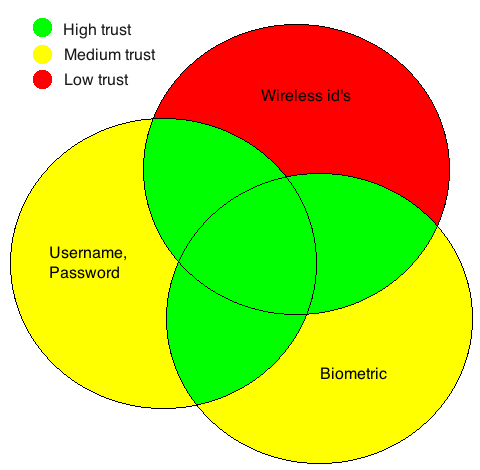
\includegraphics[width=2.5in]{img/authenticationModel}
%	\caption{ Partial login and trust }
%	\label{fig_authentication_model}
%\end{figure}
%
%High trust is obtained by authenticating with a combination of two of the three authentication methods.
%As shown in \cref{table_data_access} a user is only able to view and edit sensitive data within the high trust area of the model.
%
%Medium trust is obtained by authenticating with either a username/password or biometric authentication.
%These two authentication methods is reasonable secure and are used universally for authentication.
%A user that has obtained medium trust is able to view sensitive data but cannot edit or delete it.
%With medium trust a user can view and edit non sensitive data.
%
%Low trust is obtained by calm authentication with a Bluetooth enabled device.
%A user with low trust can view personal non sensitive data like a name or a personal todo-list.
%No edit or delete is allowed.
%
%This model allows the user to be partially authenticated before any physical interaction.
%The system gets the ability to recognize users and may for instance use that information to move a session started on one system to the current system so the user is able to seamlessly work on from the point the previous session ended.
%
%\begin{table}[!t]
%\caption{Data access}
%\label{table_data_access}
%\centering
%% Some packages, such as MDW tools, offer better commands for making tables
%% than the plain LaTeX2e tabular which is used here.
%\begin{tabular}{|p{1.3cm}|p{2.0cm}|p{2.0cm}|p{2.0cm}|}
%\hline
%\textbf{Trust} & \textbf{Non sensitive personal data} & \textbf{Non sensitive data} & \textbf{Sensitive data}\\
%\hline
%\textbf{High} & Read/Write & Read/Write & Read/Write\\
%\hline
%\textbf{Medium} & Read/Write & Read/Write & Read\\
%\hline
%\textbf{Low} & Read & - & -\\
%\hline
%\end{tabular}
%\end{table}
%

	\section{Methods}

\subsection{Existing methods}

\subsubsection{Time of Arrival (ToA)} %This sections needs more work, depending on how much descusion we need futhor on
This technology should be considered, it provides a method for measuring distance more accurately.
The technique uses the travel speed of the wireless signal to measure how far the signal travelled.
This can provide a much more accurate distance, but also has higher requirements for hardware.
It requires time synchronization which works best if hardware supported.

Support on phones and similar devices are very limited, which is why we have chosen not to look further into this method. %need ref to support claim

\url{http://en.wikipedia.org/wiki/Time_of_arrival}

\subsection{Proposed methods}

\subsection{RSSI proximity detection}

\begin{figure}[!t]
	\centering
	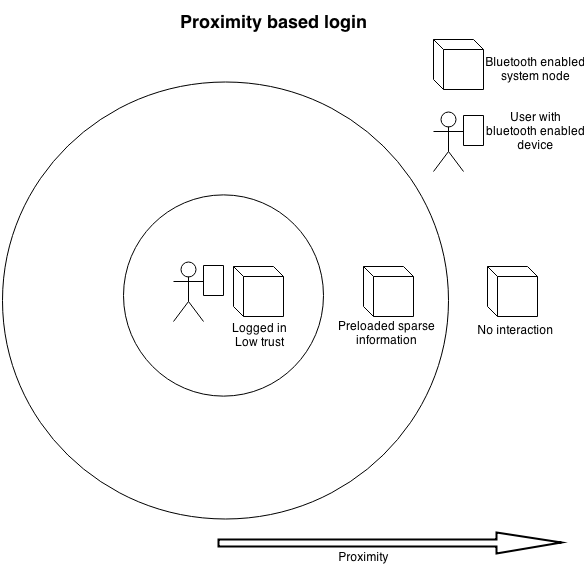
\includegraphics[width=2.5in]{img/proximityBasedLogin}
	\caption{ Proximity based login }
	\label{fig_proximity_based_login}
\end{figure}

It is hard to convert RSSI values into distance because of it's fluctuating nature and the effect of the surrounding environment. Thus instead of dealing in distances the way proximity is detected in this system is by a predefined RSSI value treshold. By determining this threshold and using filters to remove noise it is possible to use RSSI as a means for proximity detection.

When the strength of a RSSI signal reaches the predefined high threshold, when measured from the system, the user is sufficiently close to interact with the system, and the user will be partially authenticated.
When a user has been authenticated but decides to move away from the system the user will be deauthenticated when the RSSI reaches a predefined low threshold.

Furthermore it is possible to preload information about earlier sessions when a user is moving towards the system.
When the user is close enough to be partially authenticated the system thus has preloaded information and may be able to present additional relevant data based on the preloaded information from earlier sessions. 
\cref{fig_proximity_based_login} illustrates the concept of preloading information based on the users proximity to the system.

\subsection{Noise reduction filters}
In order to reduce the noise of the RSSI measurements a standard mean-filter was added to the system.

\subsection{Bluetooth Low Energy authentication}

\subsection{Partial authentication model}
A login method has been developed to take different levels of trust into account.
As presented in \cref{fig_authentication_model} the authentication model has three levels of trust
\begin{itemize}
\item High (green)
\item Medium (yellow)
\item Low (red)
\end{itemize}

\begin{figure}[!t]
	\centering
	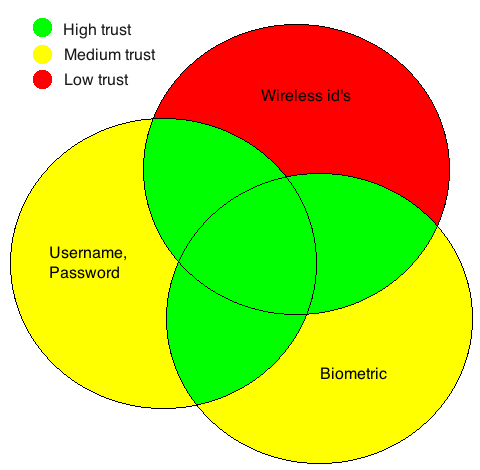
\includegraphics[width=2.5in]{img/authenticationModel}
	\caption{ Partial login and trust }
	\label{fig_authentication_model}
\end{figure}

High trust is obtained by authenticating with a combination of two of the three authentication methods.
As shown in \cref{table_data_access} a user is only able to view and edit sensitive data within the high trust area of the model.

Medium trust is obtained by authenticating with either a username/password or biometric authentication.
These two authentication methods is reasonable secure and are used universally for authentication.
A user that has obtained medium trust is able to view sensitive data but cannot edit or delete it.
With medium trust a user can view and edit non sensitive data.

Low trust is obtained by calm authentication with a Bluetooth enabled device.
A user with low trust can view personal non sensitive data like a name or a personal todo-list.
No edit or delete is allowed.

This model allows the user to be partially authenticated before any physical interaction.
The system gets the ability to recognize users and may for instance use that information to move a session started on one system to the current system so the user is able to seamlessly work on from the point the previous session ended.

\begin{table}[!t]
\caption{Data access}
\label{table_data_access}
\centering
% Some packages, such as MDW tools, offer better commands for making tables
% than the plain LaTeX2e tabular which is used here.
\begin{tabular}{|p{1.3cm}|p{2.0cm}|p{2.0cm}|p{2.0cm}|}
\hline
\textbf{Trust} & \textbf{Non sensitive personal data} & \textbf{Non sensitive data} & \textbf{Sensitive data}\\
\hline
\textbf{High} & Read/Write & Read/Write & Read/Write\\
\hline
\textbf{Medium} & Read/Write & Read/Write & Read\\
\hline
\textbf{Low} & Read & - & -\\
\hline
\end{tabular}
\end{table}
\section{Experiments}

\subsection{Test setup}

Our method requires the phone to be able to use the BLE peripheral role, and the server needs to be able to use the central role.

The specific devices used are an iPhone 5 or a Nexus 5, as mobile device and a Raspberry Pi with a Logilink USB Bluetooth 4.0 dongle running Raspbian Linux\cite{ref:raspbian} as base station. See \cref{fig_solution_overview} for an overview.

The base station test system is build as a prototype using node.js\cite{ref:node} and the Noble node module.
On the iPhone 5 we used the app LightBlue\cite{ref:Lightblue} to advertise a BLE peripheral service.

Currently BLE is amongst other supported by a number of cell phones and wearables. 
The devices tested during this research project is presented in \cref{table:devices}.

\begin{table}[!t]
\caption{Device descriptions}
\label{table:devices}
\centering
% Some packages, such as MDW tools, offer better commands for making tables
% than the plain LaTeX2e tabular which is used here.
\begin{tabular}{|p{2.3cm}|p{1.3cm}|p{3.9cm}|}
\hline
\textbf{Device} & \textbf{Hardware Support} & \textbf{Software Support}\\
\hline
iPhone 5, iPhone 5s (IOS7) & Yes & Yes\\
\hline
Nexus 5 \newline (Kitkat 4.4.2) & Yes & Partial \newline
Central role (Android 4.3)  \newline
peripheral role (Android~L)\\
\hline
Pebble Smartwatch (Pebble OS 2.0) & Yes & Peripheral role\\
\hline
Raspberry Pi (Raspian Linux) and Logilink USB Bluetooth 4.0 dongle & Yes & Yes using BlueZ stack version $\geq$ 5.0 and kernel $\geq$ 3.4\\
\hline

\end{tabular}
\end{table}

%For more information see appendix \ref{appendix:codeused}

\subsection{Scenarios}

%The base scenario consists of a Raspberry Pi with custom software as the system.
The following experiment was conducted with the base station being static throughout the experiments.

A "noisy environment" is an environment with several wifi hotspots and many people moving around with phones having access to Bluetooth, data, etc.

A "regular environment" is a standard home environment.

During the experiments there was always a clear line of sight from the mobile phone to the base station. There was no interference by physical objects or humans between the mobile phone and the base station.

%The device in the test scenario is an iPhone 5 cell phone and other wearables and will be both static and moving depending on the test scenario.

\subsubsection{Dynamic distance}
\label{section:MovingTowardsSystem}
In order for nearby authentication to work a threshold, that determines if the user is close enough for authentication, must be set.

The purpose of this scenario is to observe the relation between distance and RSSI value to make it possible to  define  this threshold. This is done by measuring the RSSI value of a single device at different distances, allowing us to define how close the user needs to be in order to be authenticated.

The base station location is constant. The phone is moved towards the system and RSSI values are measured until the device and the base station have the same location. The phone used is an iPhone 5.

This experiment was conducted in an indoor environment.


\subsubsection{Static distance}
\label{section:MovingTowardsSystem}
As mentioned, RSSI values depends on multiple factors like reflections from environment, distance, transmission strength, etc. 

The purpose of this scenario is to measure how much the RSSI value varies from a static distance. We collect data with the phone being approximately 3 meters away from the base station under the entire scenario.

The phone used is a Nexus 5 using Android L and the experiment was conducted in a regular indoor environment and in a noisy indoor environment. The purpose of the change in environment is to see how noise impacts the result.



% !TeX spellcheck = en_GB
\section{Results}
\label{sec_results}

In the following we present the results from the two scenarios.

\subsection{Dynamic distance}

\begin{figure}		
	
	\begin{tikzpicture}
\begin{axis}
[
width=0.8\textwidth,
xlabel=meter,
ylabel=dBm,
xtick={1, 2, 3, 4, 5, 6, 7, 8, 9, 10, 11, 12, 13, 14},
xticklabels={0.5, 1, 2, 3, 4, 6, 8, 10, 12, 14, 16, 18, 20},
boxplot/draw direction=y
]


%"00.5"                                
\buildBoxPlot{-50}{-46}{-59}{-73}{-43} 
%%"00"                                  
%\buildBoxPlot{-26}{-26}{-27}{-30}{-25} 
%"01"                                  
\buildBoxPlot{-55}{-54}{-58}{-63}{-47} 
%"02"                                  
\buildBoxPlot{-55}{-48}{-58}{-79}{-44} 
%"03"                                  
\buildBoxPlot{-63}{-60}{-66}{-85}{-53} 
%"04"                                  
\buildBoxPlot{-63}{-60}{-68}{-89}{-51} 
%%"05"                                  
%\buildBoxPlot{-68}{-65}{-71}{-84}{-59} 
%"06"                                  
\buildBoxPlot{-69}{-67}{-71}{-90}{-61} 
%%"07"                                  
%\buildBoxPlot{-73}{-68}{-78}{-92}{-63} 
%"08"                                  
%\buildBoxPlot{-73}{-68}{-77}{-90}{-60} 
%%"09"                                  
\buildBoxPlot{-69}{-64}{-71}{-91}{-59} 
%"10"                                  
\buildBoxPlot{-71}{-67}{-75}{-92}{-62} 
%"12"                                  
\buildBoxPlot{-78}{-75}{-82}{-94}{-66} 
%"14"                                  
\buildBoxPlot{-70}{-68}{-73}{-81}{-60} 
%"16"                                  
\buildBoxPlot{-69}{-68}{-77}{-93}{-63} 
%"18"                                  
\buildBoxPlot{-75}{-71}{-78}{-93}{-65} 
%"20"                                  
\buildBoxPlot{-77}{-74}{-80}{-91}{-66} 


\addplot[thick, red] coordinates {
	(1  ,-50)
	(2  ,-55)
	(3  ,-55)
	(4  ,-63)	
	(5  ,-63)	
	(6  ,-69)	
	(7  ,-69)
	(8  ,-71)
	(9  ,-78)
	(10 ,-70)
	(11 ,-69)
	(12 ,-75)
	(13 ,-77)
	
	};
\end{axis}


\end{tikzpicture}
	
	\caption{ Dynamic distance measurements 1 }
	\label{graf_hopper1}
	
\end{figure}

\begin{figure}		
	
	\begin{tikzpicture}
\begin{axis}
[
xlabel=meter,
ylabel=dBm,
xtick={1, 2, 3, 4, 5, 6, 7, 8, 9, 10, 11, 12, 13, 14},
xticklabels={0.5, 1, 2, 3, 4, 6, 8, 10, 12, 14, 16, 18, 20},
boxplot/draw direction=y
]


%%"00"
%\buildBoxPlot{-19}{-18}{-22}{-23}{-18}
%"00.5"
\buildBoxPlot{-43}{-42}{-45}{-49}{-41}
%"01"
\buildBoxPlot{-50}{-48}{-52}{-63}{-44}
%"02"
\buildBoxPlot{-58}{-53}{-62}{-81}{-46}
%"03"
\buildBoxPlot{-61}{-58}{-65}{-86}{-49}
%%"05"
%\buildBoxPlot{-64}{-62}{-66}{-80}{-55}
%"04"
\buildBoxPlot{-63}{-58}{-66}{-85}{-52}
%"06"
%\buildBoxPlot{-62}{-59}{-70}{-78}{-53}
%%"07"
\buildBoxPlot{-65}{-61}{-67}{-83}{-51}
%"08"
%\buildBoxPlot{-70}{-68}{-74}{-89}{-60}
%%"09"
\buildBoxPlot{-73}{-70}{-77}{-92}{-62}
%"12"
\buildBoxPlot{-62}{-61}{-64}{-75}{-57}
%"10"
\buildBoxPlot{-65}{-62}{-70}{-90}{-57}
%"16"
\buildBoxPlot{-63}{-62}{-65}{-71}{-56}
%"20"
\buildBoxPlot{-71}{-71}{-72}{-85}{-67}
%"14"
\buildBoxPlot{-68}{-64}{-71}{-81}{-57}
%"18"
\buildBoxPlot{-75}{-73}{-80}{-91}{-69}


\addplot[thick, red] coordinates {
	(1  ,-43)
	(2  ,-50)
	(3  ,-58)	
	(4  ,-61)	
	(5  ,-63)	
	(6  ,-65)
	(7  ,-73)
	(8  ,-62)
	(9 ,-65)
	(10 ,-63)
	(11 ,-71)
	(12 ,-68)
	(13 ,-75)
		
};

\end{axis}

\end{tikzpicture}
	
	\caption{ Dynamic distance measurements 2 }
	\label{graf_hopper2}
	
\end{figure}

\begin{figure}		
	
	\begin{tikzpicture}
\begin{axis}
[
xlabel=meter,
ylabel=dBm,
xtick={1, 2, 3, 4, 5, 6, 7, 8, 9, 10, 11, 12, 13, 14},
xticklabels={0.5, 1, 2, 3, 4, 6, 8, 10, 12, 14, 16, 18, 20},
boxplot/draw direction=y
]


%%"00"                                   
%\buildBoxPlot{-36}{-31}{-39}{-43}{-30}  
%"00.5"                                 
\buildBoxPlot{-55}{-50}{-61}{-83}{-46}  
%"01"                                   
\buildBoxPlot{-49}{-47}{-62}{-81}{-41}  
%"02"                                   
\buildBoxPlot{-55}{-51}{-59}{-77}{-46}  
%"03"                                   
\buildBoxPlot{-66}{-60}{-71}{-76}{-57}  
%"04"                                   
\buildBoxPlot{-60}{-55}{-62}{-65}{-52}  
%%"05"                                   
%\buildBoxPlot{-65}{-63}{-68}{-88}{-58}  
%"06"                                   
\buildBoxPlot{-66}{-65}{-68}{-78}{-59}  
%%"07"                                   
%\buildBoxPlot{-69}{-66}{-74}{-83}{-62}  
%"08"                                   
\buildBoxPlot{-63}{-62}{-75}{-83}{-59}  
%%"09"                                   
%\buildBoxPlot{-65}{-61}{-67}{-69}{-57}  
%"10"                                   
\buildBoxPlot{-63}{-62}{-65}{-72}{-57}  
%"12"                                   
\buildBoxPlot{-66}{-64}{-68}{-78}{-59}  
%"14"                                   
\buildBoxPlot{-67}{-66}{-69}{-91}{-63}  
%"16"                                   
\buildBoxPlot{-69}{-67}{-71}{-87}{-59}  
%"18"                                   
\buildBoxPlot{-73}{-71}{-76}{-88}{-65}  
%"20"                                   
\buildBoxPlot{-75}{-72}{-77}{-91}{-67}  


\addplot[thick, red] coordinates {
	(1  ,-55)
	(2  ,-49)
	(3  ,-55)	
	(4  ,-66)	
	(5  ,-60)	
	(6  ,-66)
	(7  ,-63)
	(8  ,-63)
	(9 ,-66)
	(10 ,-67)
	(11 ,-69)
	(12 ,-73)
	(13 ,-75)
	
};

\end{axis}

\end{tikzpicture}
	
	\caption{ Dynamic distance measurements 3 }
	\label{graf_hopper3}
	
\end{figure}

\begin{figure}		
	
	\begin{tikzpicture}
\begin{axis}
[
xlabel=meter,
ylabel=dBm,
xtick={1, 2, 3, 4, 5, 6, 7, 8, 9, 10, 11, 12, 13, 14},
xticklabels={0.5, 1, 2, 3, 4, 6, 8, 10, 12, 14, 16, 18, 20},
boxplot/draw direction=y
]


%%"00"                                 
%\buildBoxPlot{-13}{-12}{-15}{-16}{-10}
%"00.5"                               
\buildBoxPlot{-46}{-44}{-47}{-51}{-41}
%"01"                                 
\buildBoxPlot{-62}{-60}{-70}{-91}{-52}
%"02"                                 
\buildBoxPlot{-61}{-60}{-62}{-71}{-53}
%"03"                                 
\buildBoxPlot{-67}{-61}{-71}{-77}{-55}
%"04"                                 
\buildBoxPlot{-65}{-64}{-67}{-84}{-60}
%%"05"                                 
%\buildBoxPlot{-72}{-69}{-75}{-93}{-65}
%"06"                                 
\buildBoxPlot{-68}{-64}{-71}{-76}{-62}
%%"07"                                 
%\buildBoxPlot{-71}{-69}{-75}{-80}{-65}
%"08"                                 
\buildBoxPlot{-71}{-68}{-74}{-84}{-65}
%%"09"                                 
%\buildBoxPlot{-71}{-68}{-79}{-91}{-65}
%"10"                                 
\buildBoxPlot{-71}{-71}{-72}{-77}{-67}
%"12"                                 
\buildBoxPlot{-70}{-67}{-73}{-75}{-64}
%"14"                                 
\buildBoxPlot{-77}{-75}{-80}{-94}{-63}
%"16"                                 
\buildBoxPlot{-71}{-70}{-75}{-84}{-68}
%"18"                                 
\buildBoxPlot{-78}{-75}{-86}{-92}{-69}
%"20"                                 
\buildBoxPlot{-82}{-79}{-83}{-93}{-72} 


\addplot[thick, red] coordinates {
	(1  ,-46)
	(2  ,-62)
	(3  ,-61)	
	(4  ,-67)	
	(5  ,-65)	
	(6  ,-68)
	(7  ,-71)
	(8  ,-71)
	(9 ,-70)
	(10 ,-77)
	(11 ,-71)
	(12 ,-78)
	(13 ,-82)
	
};

\end{axis}

\end{tikzpicture}
	
	\caption{ Dynamic distance measurements 4 }
	\label{graf_hopper4}
	
\end{figure}

%\begin{figure}		
%	
%	\begin{tikzpicture}
  \begin{axis}
    [
	xlabel=meter,
	ylabel=dBm,
	xtick={1, 2, 3, 4, 5, 6, 7, 8, 9, 10, 11, 12},
    xticklabels={0, 2, 4, 6, 8, 10, 12, 14, 16, 18, 20},
    boxplot/draw direction=y
    ]
    

%"00,0"
\buildBoxPlot{-46}{ -45}{ -59}{ -63}{ -44}
%"00,5"
%\buildBoxPlot{-55}{ -55}{ -58}{ -60}{ -54}
%"01"
%\buildBoxPlot{-68}{ -67}{ -69}{ -72}{ -65}
%"02"
\buildBoxPlot{-70}{ -68}{ -74}{ -78}{ -65}
%"04"
\buildBoxPlot{-69}{ -69}{ -71}{ -72}{ -67}
%"06"
\buildBoxPlot{-78}{ -77}{ -78}{ -79}{ -73}
%"08"
\buildBoxPlot{-78}{ -77}{ -83}{ -83}{ -76}
%"10"
\buildBoxPlot{-78}{ -77}{ -79}{ -81}{ -75}
%"12"
\buildBoxPlot{-80}{ -78}{ -81}{ -84}{ -76}
%"14"
\buildBoxPlot{-77}{ -76}{ -77}{ -78}{ -75}
%"18"
\buildBoxPlot{-85}{ -83}{ -85}{ -89}{ -81}
%"16"
\buildBoxPlot{-81}{ -80}{ -81}{ -83}{ -78}
%"20"
\buildBoxPlot{-84}{ -83}{ -84}{ -87}{ -82}


\end{axis}
	
\end{tikzpicture}

%	
%	\caption{ Dynamic distance measurements Filtered }
%	\label{graf_DynamicMesurementsFiltered}
%	
%\end{figure}

The data from this scenario is presented in \cref{graf_hopper1} to \cref{graf_hopper4}.
The figure shows RSSI value at 2 meter intervals between the base station and the mobile phone.
If we look at the median of the measurements there seems to be an exponential decreasing relation between distance and RSSI value.
We also see that measurements on the low side of the mean values has a wider distribution than on the high side of the mean measurements.

\subsection{Static distance}
\begin{figure}
	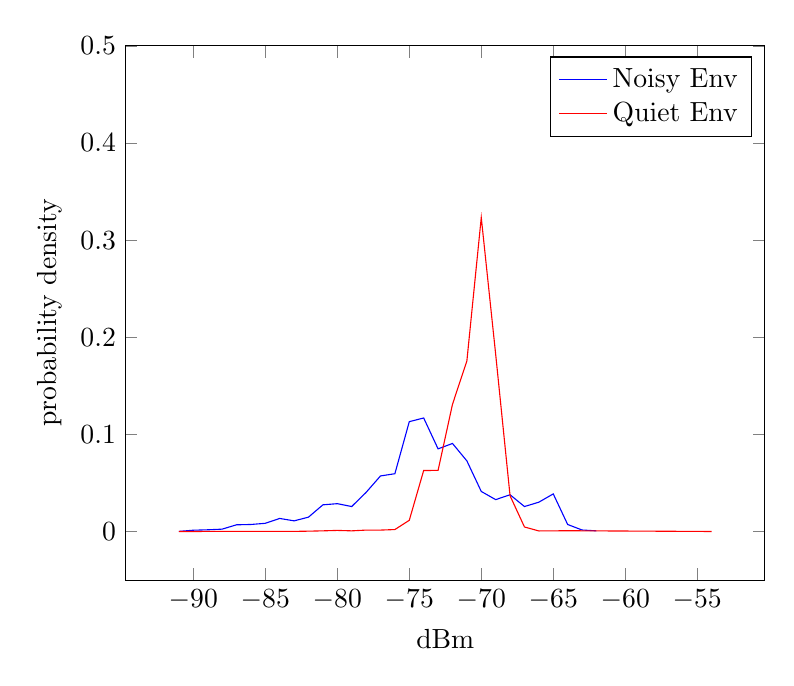
\begin{tikzpicture}
\begin{axis}[
width=0.8\textwidth,
ymax=0.5,
xlabel=dBm,
ylabel=probability density]
\addplot[blue!20!blue] coordinates {
	(-91 ,0.0001093255)
	(-90 ,0.0013119055)
	(-89 ,0.0017492074)
	(-88 ,0.0024051602)
	(-87 ,0.0068875041)
	(-86 ,0.0072154805)
	(-85 ,0.0084180606)
	(-84 ,0.0134470318)
	(-83 ,0.0109325462)
	(-82 ,0.0147589374)
	(-81 ,0.0274406909)
	(-80 ,0.028643271)
	(-79 ,0.0256914835)
	(-78 ,0.04023177)
	(-77 ,0.0571772166)
	(-76 ,0.0594730513)
	(-75 ,0.1130425276)
	(-74 ,0.1168689188)
	(-73 ,0.0850552094)
	(-72 ,0.0906308079)
	(-71 ,0.0727014322)
	(-70 ,0.0412156991)
	(-69 ,0.0327976386)
	(-68 ,0.0378266098)
	(-67 ,0.0256914835)
	(-66 ,0.0301738275)
	(-65 ,0.0387012135)
	(-64 ,0.0072154805)
	(-63 ,0.0015305565)
	(-62 ,0.0006559528)

		};
\addplot[red!20!red] coordinates {
	(-91, 0)
	(-87, 0.0001107297)
	(-86, 0.0001107297)
	(-83, 0.0001107297)
	(-82, 0.0003321891)
	(-81, 0.0006643783)
	(-80, 0.0011072971)
	(-79, 0.0006643783)
	(-78, 0.0014394862)
	(-77, 0.0014394862)
	(-76, 0.0019931348)
	(-75, 0.0115158897)
	(-74, 0.0627837449)
	(-73, 0.0628944746)
	(-72, 0.1308825158)
	(-71, 0.1755065884)
	(-70, 0.3232200199)
	(-69, 0.1824825601)
	(-68, 0.0367622633)
	(-67, 0.0046506478)
	(-66, 0.0005536485)
	(-64, 0.000775108)
	(-54, 0)
	};
\legend{Noisy Env,Quiet Env}
\end{axis}
\end{tikzpicture}

	
	\caption{Static distance measurements}
	\label{graf_StaticMesurements}
\end{figure}

The data from this scenario is presented in \cref{graf_StaticMesurements}.
The figure shows how measurements are distributed over a period of 20 minutes when the distance between the base station and the mobile phone is static.
The experiment was performed in a quiet and a noisy environment.
As one would expect the RSSI values has a much higher spread in the noisy environment than in the quiet environment. 
 

\section{Discussion}
Seeing how the value of the RSSI measured from the device fluctuates in \cref{graf_hopper1} to \cref{graf_hopper4} it is clear that RSSI is hard to use for distance measurements.
From a mean around 45 when measured right on top of the system the RSSI value drops drastically within the first few meters.
As the device moves further away from the system the RSSI value becomes lower but there is no apparent model to the decline.

The noise seams to fluctuate more towards the noise side of the mean. This suggests that if a lower value is measured it is more reliable then a high value, witch fits in well for authentication purposes.
Since most outliers are in the lower dBm end, there is a greater chance that you will be incorrectly logged out as a result of noise than incorrectly logged in.

Looking at \cref{graf_StaticMesurements} we clearly see that the RSSI value becomes less reliable the more noise there is in the environment.
The Noise level will affect how the hysteresis thresholds should be configured.
With too much noise in the environment the mean value of the graph will become indistinct from the rest.




\section{Conclusion}
Using RSSI value as viable means for proximity detection is possible but inaccurate. Therefore we implemented a solution which uses a filter and a hysteresis threshold combined, to remove noise from RSSI measurements and optimize accuracy and thereby make a more consistent proximity detection.

RSSI values depends on multiple factors, such as distance, reflections from environment, transmission strength, etc., which is reflected in our test results.
Environment knowledge prior to implementing authentication using RSSI values is therefore crucial to be able to calibrate the base station correctly. 
Even when the base station is calibrated there is the possibility of interference of for instance people moving between the mobile phone and the base station. 
This adds a layer of inaccuracy to the system which is really hard to predict and therefore take into account when doing proximity detection.

We have developed an application that is capable of proximity detecting of a BLE device running with the peripheral role. This is done using the RSSI value witch is being broadcasted by the device.

Because RSSI measurements are significantly effected by the environment, hysteresis thresholds must be used and calibrated with respect to the environment.
We have found that this method makes authentication possible using BLE, however for a highly secured system this method might not be secure enough.

Source code is available on Github:
\url{https://github.com/KrauseStefan/ReserchProject-RSSI-Login/tree/master/testApp}.

%
%A partial authentication model has been proposed taking the security aspect of calm authentication into consideration. The model has three levels of trust: Low, Medium and High allowing different read/write/edit rights according to the level of trust.

%We have shown that context aware authentication using Bluetooth Low Energy is possible using RSSI measurements for proximity detection.



% if have a single appendix:
%\appendix[Proof of the Zonklar Equations]
% or
%\appendix  % for no appendix heading
% do not use \section anymore after \appendix, only \section*
% is possibly needed

% use appendices with more than one appendix
% then use \section to start each appendix
% you must declare a \section before using any
% \subsection or using \label (\appendices by itself
% starts a section numbered zero.)
%


\appendices
\section{Proof of the First Zonklar Equation}
Appendix one text goes here.

% you can choose not to have a title for an appendix
% if you want by leaving the argument blank
\section{}
Appendix two text goes here.


% use section* for acknowledgement
\ifCLASSOPTIONcompsoc
  % The Computer Society usually uses the plural form
  \section*{Acknowledgments}
\else
  % regular IEEE prefers the singular form
  \section*{Acknowledgment}
\fi


The authors would like to thank...


% Can use something like this to put references on a page
% by themselves when using endfloat and the captionsoff option.
\ifCLASSOPTIONcaptionsoff
  \newpage
\fi


% references section

% can use a bibliography generated by BibTeX as a .bbl file
% BibTeX documentation can be easily obtained at:
% http://www.ctan.org/tex-archive/biblio/bibtex/contrib/doc/
% The IEEEtran BibTeX style support page is at:
% http://www.michaelshell.org/tex/ieeetran/bibtex/
%\bibliographystyle{IEEEtran}
% argument is your BibTeX string definitions and bibliography database(s)
%\bibliography{IEEEabrv,../bib/paper}
%
% <OR> manually copy in the resultant .bbl file
% set second argument of \begin to the number of references
% (used to reserve space for the reference number labels box)
\begin{thebibliography}{1}

\bibitem{ref:Takashi}
 Kikawa, Yoshikawa, Ohkubo, Takeshita, Shiraishi and Takahashi:  
 A Presence-detection Method using RSSI of a Bluetooth Device, 2010, International Journal of Informatics Society, VOL. 2, NO. 1. 

%\bibitem{ref:win8_BLE_support}
%Bluetooth Low Energy Overview. Microsoft developer network. Retrieved from http://msdn.microsoft.com/en-us/library/windows/hardware/jj159880(v=vs.85).aspx

\bibitem{ref:Power_usage}
iBeacon Battery Drain on Apple vs Android: A Technical Report. Aislelabs. Retrieved from http://www.aislelabs.com/reports/ibeacon-battery-drain-iphones/

\bibitem{ref:bardram}
E. Bardram. 2005. The trouble with login: on usability and computer security in ubiquitous computing. Personal Ubiquitous Comput. 9, 6 (November 2005), 357-367. DOI=10.1007/s00779-005-0347-6 http://dx.doi.org/10.1007/s00779-005-0347-6

\bibitem{ref:covington}
Covington, Michael J., et al. "A context-aware security architecture for emerging applications." Computer Security Applications Conference, 2002. Proceedings. 18th Annual. IEEE, 2002.

\bibitem{ref:bandara}
Bandara, Udana, et al. "Design and implementation of a bluetooth signal strength based location sensing system." Radio and Wireless Conference, 2004 IEEE. IEEE, 2004.

\bibitem{ref:rssidistance}
Awad, Abdalkarim, Thorsten Frunzke, and Falko Dressler. "Adaptive distance estimation and localization in WSN using RSSI measures." Digital System Design Architectures, Methods and Tools, 2007. DSD 2007. 10th Euromicro Conference on. IEEE, 2007.

\bibitem{ref:node}
Tilkov, Stefan, and Steve Vinoski. "Node. js: Using JavaScript to build high-performance network programs." IEEE Internet Computing 14.6 (2010): 0080-83.

\bibitem{ref:Lightblue}
https://itunes.apple.com/dk/app/lightblue-bluetooth-low-energy/id557428110?mt=8

\bibitem{ref:raspbian}
http://www.raspbian.org/

%H.~Kopka and P.~W. Daly, \emph{A Guide to \LaTeX}, 3rd~ed.\hskip 1em plus
%  0.5em minus 0.4em\relax Harlow, England: Addison-Wesley, 1999.

\end{thebibliography}


% trigger a \newpage just before the given reference
% number - used to balance the columns on the last page
% adjust value as needed - may need to be readjusted if
% the document is modified later
%\IEEEtriggeratref{8}
% The "triggered" command can be changed if desired:
%\IEEEtriggercmd{\enlargethispage{-5in}}

\include*{sections/B_Biography}


% that's all folks
\end{document}

